\chapter{Erstes Kapitel}
Dies ist eine Vorlage für wissenschaftliche Arbeiten an der FHGR nach \cite{selina_leitfaden_nodate}. Wörter kann man auch abkürzen: \ac{zb}, \ac{etc}. Die folgende Abbildung zeigt eine Alpendohle (Abb. \ref{fig:alpendohle}).

\begin{figure}[h]
    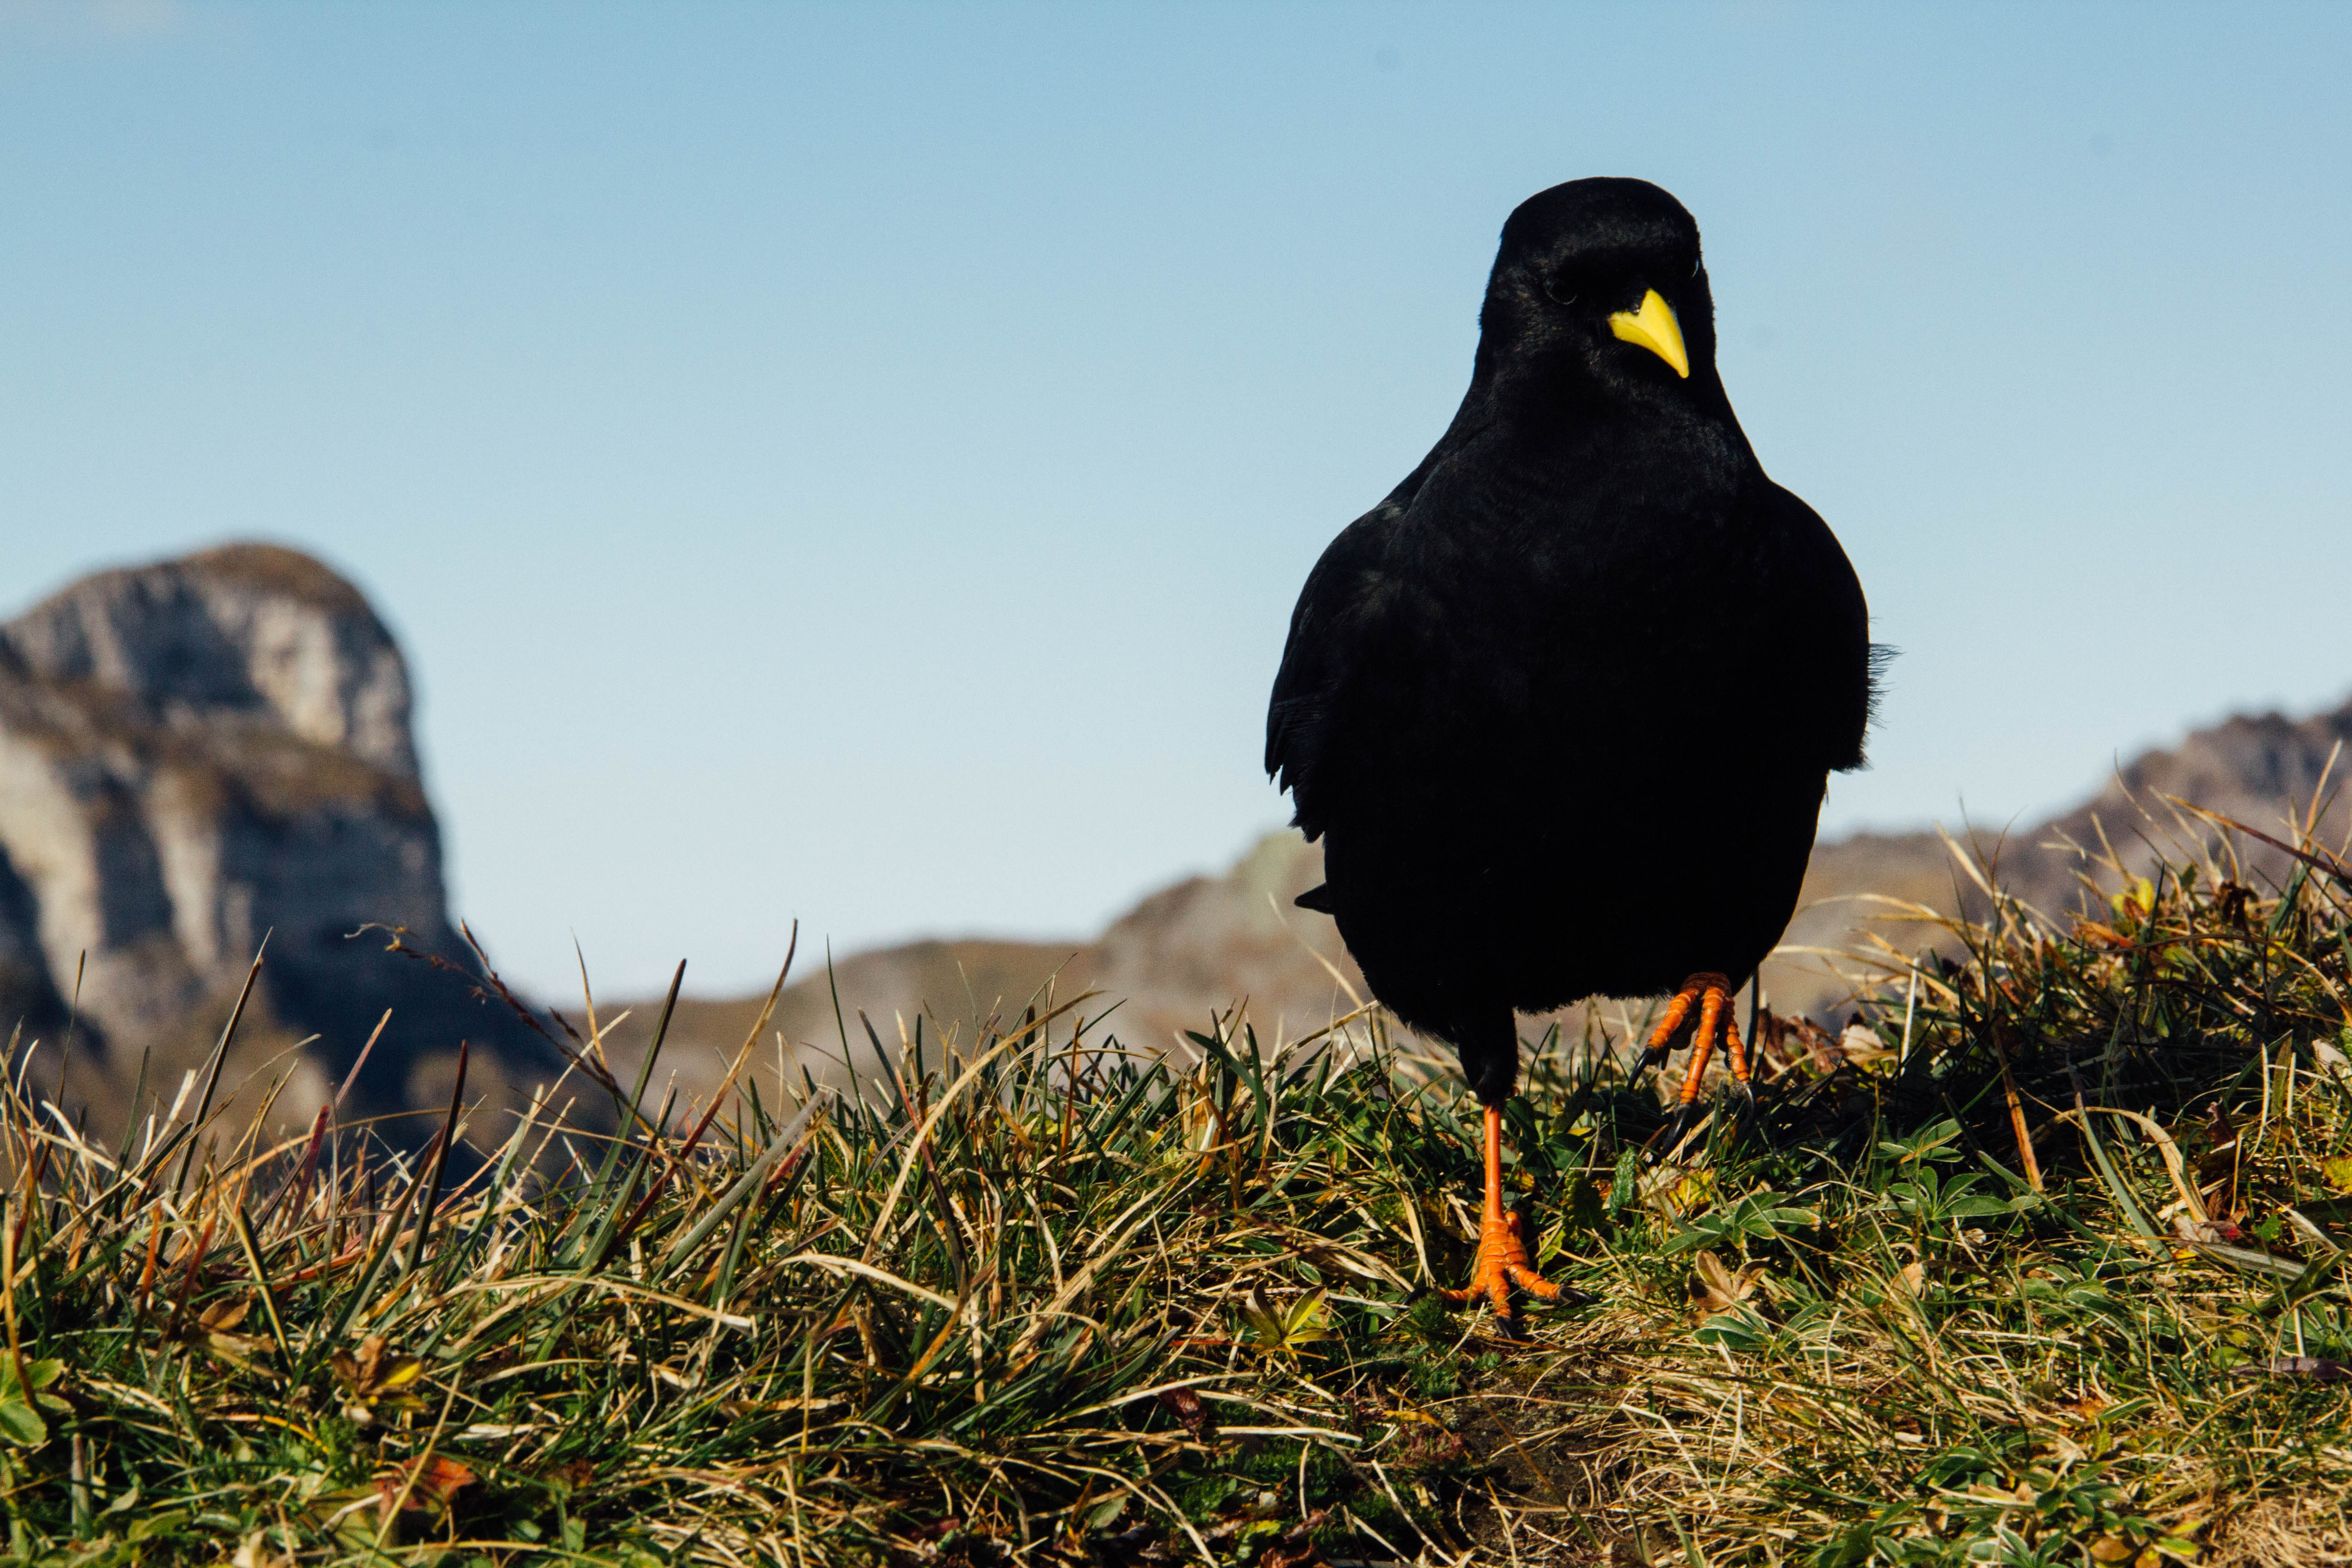
\includegraphics[width=\textwidth]{content/00_assets/alpendohle.jpg}
    \caption{Eine Alpendohle \citep{diani_black_2016}}
    \label{fig:alpendohle}
\end{figure}

\blindtext

\begin{table}[ht]
\begin{tabularx}{\textwidth} {
    >{\raggedright\arraybackslash}X 
    >{\raggedleft\arraybackslash}X 
    >{\raggedleft\arraybackslash}X}
        \hline
        \multicolumn{3}{c}{\textbf{Tabelle}}\\
        \hline
        \textbf{Linksbündig} & \textbf{Rechtsbündig} & \textbf{Rechtsbündig}\\
        \hline
        Lorem & N/A & N/A\\
        Ipsum & 1 499 & 8 512\\
        Dolor & 297 & N/A\\
        Sit & 1 053 & N/A\\
        \hline
        \textbf{Total} & 2 849 & 8 512\\
        \hline
\end{tabularx}
\caption{Beispiel einer Tabelle}.
    \label{tab:tabelle}
\end{table}

\section{Subkapitel}
\blindtext

\section{Subkapitel}
\blindtext
\begin{quote}
    \blindtext
\end{quote}
\blindtext